\documentclass[10pt]{article}
\usepackage{amsmath,textcomp,amssymb,geometry,graphicx,enumerate,tikz,algorithm,algpseudocode,pifont}
\usetikzlibrary{calc}
\usetikzlibrary{datavisualization}
\usetikzlibrary{datavisualization.formats.functions}


\textheight=9in
\textwidth=7in
\topmargin=-.75in
\oddsidemargin=-0.25in
\evensidemargin=-0.25in

\usepackage{listings}
\lstnewenvironment{codeblock}
    {\lstset{language=Python,
      showspaces=false,
      showtabs=false,
      breaklines=true,
      mathescape=true,
      showstringspaces=false,
      breakatwhitespace=true,
      commentstyle=\textit,
      keywordstyle=\textbf,
      basicstyle=\ttfamily,
      escapechar=`,
      moredelim={**[is][{\color{RoyalBlue}}]{\^^M\\beginsol}{\^^M\\endsol}},
      moredelim={[is][{\color{RoyalBlue}}]{\^^M\\beginexp}{\^^M\\endexp}},
    }}
    {}

\begin{document}
\section*{03/14/2016}
\subsection*{Decision Trees}
	\begin{itemize}
		\item Non-linear method for classification.
		\item Uses trees with two node types:
			\begin{itemize}
				\item internal nodes test feature values (usually just one) and branch accordingly.
				\item leaf nodes specify class $h(x)$.	
				\begin{center}
					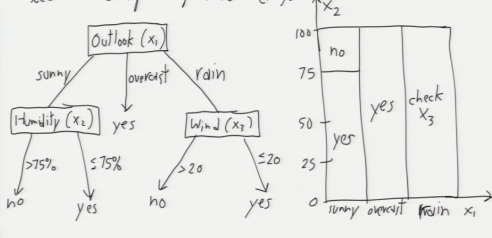
\includegraphics[scale=0.6]{../images/tree:graph}
				\end{center}
			\end{itemize}
		\item Cuts x-space into rectangular cells.
		\item Works well with both categorical and quantitative features.
		\item Interpretable result (inference).
		\item Decision boundary can be arbitrarily complicated.
			\begin{itemize}
				\item Can really reduce bias if boundary is truly complicated.
				\item A lot of opportunity for over-fitting.
				\begin{center}
					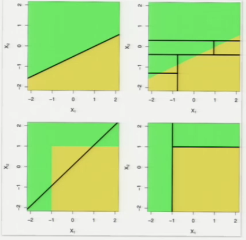
\includegraphics[scale=0.8]{../images/decisiontreeexamples}
				\end{center}
			\end{itemize}
		\item Leaf is pure if every training sample in it has the same class.
		\item Consider classification first: Greedy, top-down learning heuristic: 
		\item Let $S \subseteq \{1, 2, \dots, n\}$ be a list of sample indices.
		\item Top level call: $S = \{1, 2, \dots, n\}$
		\end{itemize}
\begin{codeblock}
	GrowTree($S$):
	    if ($y_{i} = c \ \forall i \in S$ and some class C):
	        return new leaf(C)
	    else:
	        choose best splitting feature $j$ and splitting point $\beta$ (*)
	        $S_{\ell} = \{i : X_{ij} < \beta \}$
	        $S_{r} = \{ : X_{ij} \geq \beta \}$
	        return new node($j, \beta, $GrowTree$(S_{\ell}), $GrowTree$(S_{r}))$
\end{codeblock}
	\begin{itemize}
		\item (*) How to choose best split?
			\begin{itemize}
				\item Try all splits.
				\item For a set $S$, let $J(S)$ be the \underline{cost} of $S$.
				\item Choose the split that minimizes $J(S_{\ell}) + J(S_{r})$; or, the split that minimizes the weighted average $\frac{|S_{\ell}|J(S_{\ell})+ |S_{r}|J(S_{r})}{|S_{\ell}| + |S_{r}|}$
			\end{itemize}
		\item How to choose cost $J(S)$?
			\begin{itemize}
				\item Idea 1 (bad): Label $S$ with the class $C$ that labels the most samples in $S$. $J(S) \leftarrow$ number of samples in $S$ not in class $C$.
				\begin{center}
					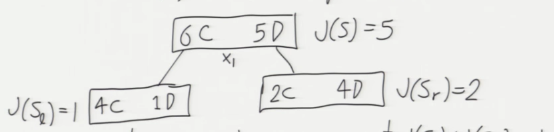
\includegraphics[scale=0.6]{../images/idea1good}
				\end{center}
				\begin{itemize}
					\item Problem: sometimes we make "progress," yet $J(S_{\ell}) + J(S_{r}) = J(S)$.
				\begin{center}
					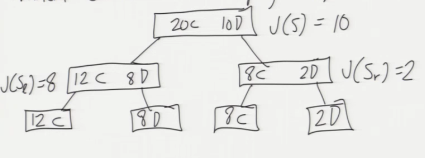
\includegraphics[scale=0.6]{../images/idea1bad}
				\end{center}
				\end{itemize}
				\item Idea 2 (good): Measure \underline{entropy}.
				\begin{itemize}
					\item Let $Y$ be a random class variable, and suppose $P(Y=C) = p_{c}$.
					\item The \underline{surprise} of $Y$ being class $C$ is $S(Y=C) = -log_{2} \ p_{c}$.
						\begin{itemize}
							\item event with probability 1 gives us zero surprise.
							\item event with probability 0 gives us infinite surprise.
						\end{itemize}
					\item The \underline{entropy} of an index set $S$ is the average surprise: $H(S) = -\sum_{c} p_{c} \ log_{2} \ p_{c}$, where $p_{c} = \frac{|\{i \in S : y_{i} = C\}|}{|S|}$
					\item If all samples in $S$ belong to same class? $H(S) = -1 \ log_{2} \ 1 = 0$.
					\item Half class $C$, half class $D$? $H(S) = -\frac{1}{2} \ log_{2} \frac{1}{2} - \frac{1}{2} \ log_{2} \frac{1}{2} = 1$.
					\item n samples, all different classes? $H(S) = -log_{2} \ \frac{1}{n} = log_{2} \ n$.
					\begin{center}
						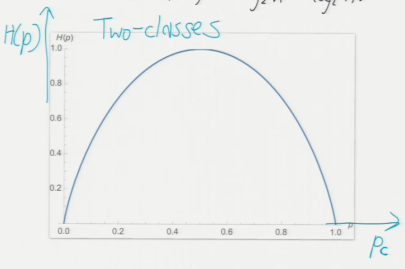
\includegraphics[scale=0.7]{../images/entropy}
					\end{center}
				\end{itemize}
				
			\item Weighted average entropy after split is $H_{after} = \frac{|S_{\ell}|H(S_{\ell})+ |S_{r}|H(S_{r})}{|S_{\ell}| + |S_{r}|}$
			\item Choose split that maximizes \underline{information gain} $H(S) - H_{after}$.
			\begin{center}
				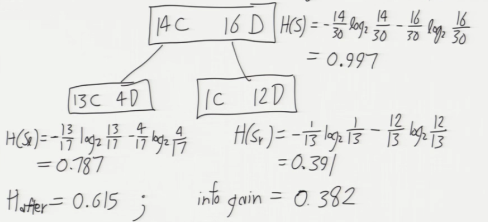
\includegraphics[scale=0.6]{../images/informationgain}
			\end{center}
			\item Information gain always positive expect when one child is empty or \\ $\ \forall C, P(y_{i} = C|i \in S_{\ell}) = P(y_{i}=C|i \in S_{r})$ 
			\begin{center}
				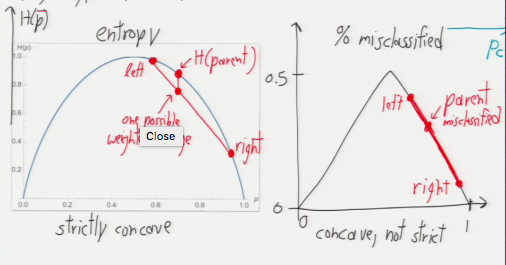
\includegraphics[scale=0.7]{../images/idea1vsidea2}
			\end{center}
			\end{itemize}
		\item More on choosing a split.
			\begin{itemize}
				\item For binary feature $x_{i}$, children are $x_{i}=0$ and $x_{i}  =1$.
				\item If $x_{i}$ has 3+ discrete values, split depends on application.
				\item If $x_{i}$ is quantitative, sort samples in $S$ by feature $x_{i}$; remove duplicates try splitting between each pari of consecutive samples.
				\item Clever Bit: As you scan sorted list from left to right, you can update entropy in $\mathcal{O}(1)$ time per sample!
				\begin{center}
					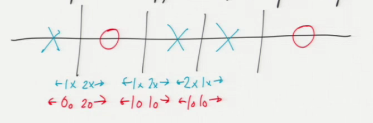
\includegraphics[scale=0.6]{../images/binarysplits}
				\end{center}
			\end{itemize}
		\item Algorithms and running times:
			\begin{itemize}
				\item Test point: walk down tree until leaf. Return it's label.
				\begin{itemize}
					\item Worst-case time is $\mathcal{O}(\text{depth tree})$.
					\item For binary features, that's $\leq d$.
					\item Usually (not always) $\leq \mathcal{O}(\log n)$.
				\end{itemize}
				\item Training:
				\begin{itemize}
					\item For binary features, try $\mathcal{O}(d)$ splits at each node.
					\item For quantitative features, try $\mathcal{O}(n'd)$ splits; $n' =$ samples in node.
					\item Either way, $\Rightarrow \mathcal{O}(n'd)$ time at this node.
				\end{itemize}
				\item Each sample participates in $\mathcal{O}(\text{depth})$ nodes, cost $\mathcal{O}(d)$ time in each node.
				\item Running time $\leq \mathcal{O}(dn \text{depth})$.
			\end{itemize}
	\end{itemize}	
\end{document}
